% Torture deck for text fit: every frame is one way a line can come out of Slides wider or
% narrower than the PDF drew it (the substitute font, its size, its letters, the room around
% it), and what that does next - a wrap, a table that grows over its caption, a centred title
% leaning off its axis, a line running into its neighbour. Measured on Google's renderer by
% tools/text_fit.py after `convert` and `fidelity` (docs/project-notes.md, "Text fit").
\documentclass{beamer}
\usetheme{Madrid}
\usepackage{booktabs}
\usepackage{multirow}
\usepackage{pgfplots}
\pgfplotsset{compat=1.18}
\setbeamertemplate{caption}[numbered]
\title{Text fit}
\author{Torture}

\newcommand{\probe}{Monitor Workstation Mainframe 12,345.67}

\begin{document}

\begin{frame}[label=sizes-left]{Sizes, left}
  {\tiny \probe\par}
  {\scriptsize \probe\par}
  {\footnotesize \probe\par}
  {\small \probe\par}
  {\normalsize \probe\par}
  {\large \probe\par}
  {\Large \probe\par}
  {\LARGE Monitor Workstation 12,345\par}
  {\huge Monitor 12,345\par}
\end{frame}

\begin{frame}[label=sizes-centred]{Sizes, centred}
  \begin{center}
    {\tiny \probe\par}
    {\footnotesize \probe\par}
    {\normalsize \probe\par}
    {\Large \probe\par}
    {\huge Monitor 12,345\par}
  \end{center}
\end{frame}

\begin{frame}[label=sizes-right]{Sizes, flush right}
  \begin{flushright}
    {\tiny \probe\par}
    {\footnotesize \probe\par}
    {\normalsize \probe\par}
    {\Large \probe\par}
    {\huge Monitor 12,345\par}
  \end{flushright}
\end{frame}

\begin{frame}[label=faces]{Faces and letters}
  {\rmfamily Serif: Monitor Workstation Mainframe WWWW MMMM\par}
  {\ttfamily Typewriter: Monitor Workstation 12,345\par}
  {\bfseries Bold: Monitor Workstation Mainframe WWWW\par}
  {\itshape Italic: Monitor Workstation Mainframe WWWW\par}
  {\scshape Small caps: Monitor Workstation Mainframe\par}
  {\bfseries\itshape Bold italic: Monitor Workstation WWWW\par}
  Wide letters: WWWWWWWW MMMMMMMM mmmmmmmm wwwwwwww\par
  Narrow letters: illicit ill-fitting little lilies liftlift\par
  Digits: 0123456789 1,111,111.11 8,888,888.88 100\%\par
\end{frame}

\begin{frame}[label=full-width]{A paragraph filling the width}
  The substitute font is a few per cent wider than Computer Modern, so a justified paragraph
  whose lines are full in the PDF has to break somewhere else in Slides unless the box leaves
  room. Every line here is as long as the text width allows, which is exactly the case where
  a word at the end of a line drops onto the next one and the paragraph grows by a line.

  \small A second paragraph in a smaller size fills its lines too, and must keep the number of
  lines it has in the PDF: otherwise everything below it moves down on the slide.
\end{frame}

\begin{frame}[label=columns]{Two full columns}
  \begin{columns}[T]
    \column{0.48\textwidth}
    A column of justified text that fills its whole width, set close to the other column so
    the gutter between them is the only room a wider font has.
    \column{0.48\textwidth}
    \raggedleft The right column is set flush right, so a wider font grows towards the left
    edge, into the gutter, and toward the words of the left column.
  \end{columns}
\end{frame}

\begin{frame}[label=items]{Items near the edge}
  \begin{itemize}
    \item An item whose words run almost to the right edge of the text area here
    \item Short item
    \begin{itemize}
      \item A nested item that is long enough to fill the narrower nested measure too
      \item Monitor Workstation Mainframe 12,345.67 Monitor Workstation
    \end{itemize}
    \item \textbf{Bold item that fills most of the line at normal size}
  \end{itemize}
  \begin{enumerate}
    \item Numbered item with a long line that reaches the right-hand margin
  \end{enumerate}
\end{frame}

\begin{frame}[label=description]{Description labels}
  \begin{description}[Workstation]
    \item[Monitor] a label shorter than the widest one
    \item[Workstation] the widest label decides where every text starts
    \item[Mainframe] and a text that runs on long enough to reach the margin here
  \end{description}
\end{frame}

\begin{frame}[label=blocks]{Blocks}
  \begin{block}{A block title long enough to fill the title bar of the block}
    Block body text that fills the width of the block, right up to its edge, twice over:
    a wider font must not push the last word outside the coloured panel.
  \end{block}
  \begin{exampleblock}{Short}
    \centering Centred body: Monitor Workstation Mainframe
  \end{exampleblock}
\end{frame}

\begin{frame}[label=table-tight]{Tight numeric table}
  \begin{table}
    \centering\footnotesize
    \begin{tabular}{@{}llrr@{}}
      \toprule
      Dataset & Split & Images & Classes \\
      \midrule
      ImageNet-1k & train & 1,281,167 & 1000 \\
      ImageNet-1k & val & 50,000 & 1000 \\
      Places365 & train & 1,803,460 & 365 \\
      Monitor & Workstation & 12,345,678 & 99 \\
      \bottomrule
    \end{tabular}
    \caption{Numbers are wider in the substitute font.}
  \end{table}
\end{frame}

\begin{frame}[label=table-header]{Large bold header}
  \begin{table}
    \centering\large
    \begin{tabular}{lccc}
      \toprule
      \textbf{Monitor} & \textbf{Workstation} & \textbf{Mainframe} & \textbf{Total} \\
      \midrule
      mmm & www & 1,234 & 5,678 \\
      iii & lll & 9,999 & 0,000 \\
      \bottomrule
    \end{tabular}
    \caption{A bold header in a large size.}
  \end{table}
\end{frame}

\begin{frame}[label=table-merged]{Merged header and wrapped cell}
  \begin{table}
    \centering\small
    \begin{tabular}{lp{3.2cm}rr}
      \toprule
      & & \multicolumn{2}{c}{Test results} \\
      \cmidrule(l){3-4}
      Method & Notes (wrapped on purpose) & BLEU & Time \\
      \midrule
      Baseline & A cell set in a paragraph column, which wraps in the PDF too & 27.3 & 12h \\
      Ours & Short note & 31.0 & 14h \\
      \bottomrule
    \end{tabular}
    \caption{Translation quality on newstest2014, with a caption long enough to fill the line.}
  \end{table}
\end{frame}

\begin{frame}[label=table-wide]{Wide numbers, no side bearings}
  \centering
  \begin{tabular}{@{}lrrr@{}}
    \hline
    Quarter & Revenue & Cost & Margin \\
    \hline
    Q1 2026 & 12,345,678.90 & 9,876,543.21 & 24.98\% \\
    Q2 2026 & 13,579,246.80 & 10,864,197.53 & 19.99\% \\
    \hline
  \end{tabular}

  \vspace{4pt}
  Text right under the table: it must stay clear of the last row.
\end{frame}

\begin{frame}[label=chart]{Chart with long ticks}
  \begin{figure}
    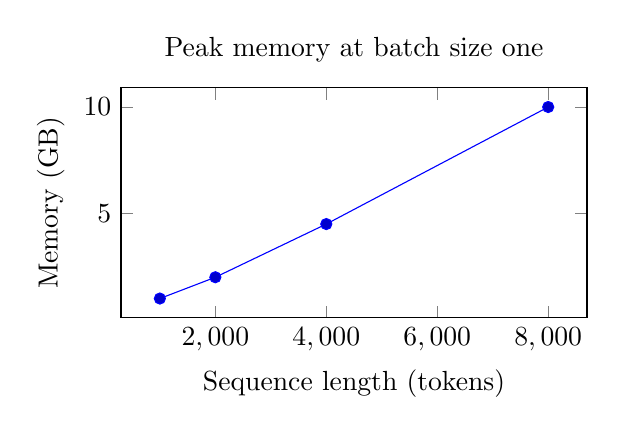
\begin{tikzpicture}
      \begin{axis}[width=7.5cm, height=4.5cm, xlabel={Sequence length (tokens)},
          ylabel={Memory (GB)}, title={Peak memory at batch size one},
          xticklabel style={/pgf/number format/1000 sep={,}}]
        \addplot coordinates {(1000,1) (2000,2) (4000,4.5) (8000,10)};
      \end{axis}
    \end{tikzpicture}
    \caption{The caption under a chart stays text.}
  \end{figure}
\end{frame}

\begin{frame}[label=beside]{Text beside a figure}
  \begin{columns}[c]
    \column{0.45\textwidth}
    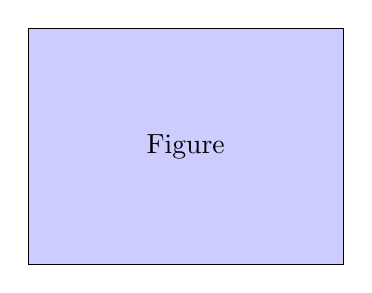
\begin{tikzpicture}
      \draw[fill=blue!20] (0,0) rectangle (4,3);
      \node at (2,1.5) {Figure};
    \end{tikzpicture}
    \column{0.5\textwidth}
    Text set right beside the figure, so that a wider font runs toward the next column and
    wraps where the PDF did not.
  \end{columns}
\end{frame}

\begin{frame}[label=edges]{Against the edges}
  \hfill\Large Monitor Workstation Mainframe\par
  \vfill
  \tiny A line of tiny text at the bottom of the frame, set as wide as the text width allows,
  with no room at all to its right: Monitor Workstation Mainframe 12,345.67 and more words.
\end{frame}

\begin{frame}[label=inline-math]{Inline math in a full line}
  With $x_1^2 + y_1^2 = r^2$ and $\alpha_{t+1} = \alpha_t - \eta \nabla L(\theta_t)$ in the
  same line, the scripts and symbols are set in other fonts, and the line is still full.

  Sums like $\sum_i w_i x_i$ and ratios like $a/b$ keep their line as well.
\end{frame}

\begin{frame}[label=numbers]{Numbers and signs}
  \begin{itemize}
    \item \$1,234,567.89 \quad EUR 98.76 \quad 3.14159 \quad 100\% \quad 2026-09-23
    \item 12:45:30 \quad v1.2.3-rc4 \quad 192.168.0.1 \quad \#42 \quad x86\_64
    \item {\ttfamily 0x7fff\_ffff \quad 1e-9 \quad [0, 1) \quad a->b}
  \end{itemize}
\end{frame}

\end{document}
